\documentclass{beamer}
\usepackage{amsmath}
\usepackage{graphicx}

\usetheme{Warsaw}

\title{Double Fourier Series}
\author{Kaustubh Dandegaonkar, Himanshu Jindal, Shubham Vishwakarma}
\date{\today}

\begin{document}

\frame{\titlepage}


\begin{frame}
\frametitle{Fourier series in 1-D}
\begin{itemize}
    \item A periodic function $f(x)$ with a period of $1$ and for which $\int_{0}^{1} f(x)^2 \,dx$ is finite has a Fourier series expansion:
    \[ f(x) \sim \frac{a_0}{2} + \sum_{n=1}^{\infty} \left( a_n \cos (2\pi nx) + b_n \sin(2\pi nx) \right) \]
    \item If $f(x)$ is continuously differentiable, its Fourier series converges uniformly.
\end{itemize}
\end{frame}


\begin{frame}
\frametitle{Fourier series in higher dimensions (vector notation)}
\begin{itemize}

    \item Consider a function $f(x_1, x_2)$ $(p_1, p_2)$-periodic in variables $x_1$ and $x_2$.
    \item Assuming $p_1$ and $p_2$ to be 1, the condition is:
    \[ f(x_1 + n_1, x_2 + n_2) = f(x_1, x_2) \quad \forall x_1, x_2 \in [0, 1] \]
    \item Using vector notation, $x = (x_1, x_2)$ and $n = (n_1, n_2)$, the condition becomes:
    \[ f(x+n) = f(x) \quad  n \in \mathbb{N} \]
\end{itemize}
\end{frame}

\begin{frame}
\frametitle{Fourier series in higher dimensions (vector notation)}
\begin{itemize}

    \item In 2-D, the building blocks for periodic function $f(x_1, x_2)$ are the product of complex exponentials in one variable.
    \item The general higher harmonic is of the form:
    \[ e^{2\pi in_1 x_1} e^{2\pi in_2 x_2} \]
    \item We can write the Fourier series expansion as:
    \[ \sum_{n_1, n_2} c_{n_1, n_2} e^{2\pi i (n_1 x_1 + n_2 x_2)} \]
\end{itemize}
\end{frame}


\begin{frame}
\frametitle{Fourier series in 2-D }
\begin{itemize}

    \item Let $f(x, y)$ be a continuously differentiable periodic function with a period of $1$ in both variables.
    \item For each value of $y$, we can expand $f(x, y)$ in a uniformly convergent Fourier series:
    \begin{align*}
    f(x,y) = a_{0}+ \sum b_{m}\cos(2\pi mx)+\sum c_{m}\sin(2\pi mx)\\
    &\hspace{-17em} +\sum d_{n}\cos\left(2\pi ny\right)+\sum e_{n}\sin\left(2\pi ny\right)\\
    &\hspace{-17em} +\sum\sum f_{mn}\cos\left(2\pi mx\right)\sin\left(2\pi ny\right)\\
    &\hspace{-17em} +\sum\sum g_{mn}\cos\left(2\pi mx\right)\cos\left(2\pi ny\right)\\
    &\hspace{-17em} +\sum\sum h_{mn}\sin\left(2\pi mx\right)\sin\left(2\pi ny\right)\\
    &\hspace{-17em} +\sum\sum k_{mn}\sin\left(2\pi mx\right)\cos\left(2\pi ny\right)
    \end{align*}
    
\end{itemize}
\end{frame}

\begin{frame}{Fourier series in 2-D}
    \begin{itemize}
        \item where,
        \begin{align*}
            &\hspace{-12em}a_{0}=\int\limits_{0}^{1}\int\limits_{0}^{1}f\left(x,y\right)dxdy\\
            &\hspace{-12em}b_{m}=2\int_{0}^{1}\int_{0}^{1}f(x,y)\cos(2\pi mx)dxdy\\
            &\hspace{-12em}c_{m}=2\int_{0}^{1}\int_{0}^{1}f(x,y)\sin(2\pi mx)dxdy\\
            &\hspace{-12em}d_{n}=2\int_{0}^{1}\int_{0}^{1}f(x,y)\cos(2\pi ny)dxdy\\
            &\hspace{-12em}e_{n}=2\int_{0}^{1}\int_{0}^{1}f(x,y)\sin(2\pi ny)dxdy\\
        \end{align*}
    \end{itemize}
\end{frame}

\begin{frame}{Fourier Series in 2D}
\begin{align*}
    f_{mn}=4\int_{0}^{1}\int_{0}^{1}f(x,y)\cos(2 \pi mx)\sin(2\pi ny)dxdy\\
    g_{mn}=4\int_{0}^{1}\int_{0}^{1}f(x,y)\cos(2 \pi mx)\cos(2\pi ny)dxdy\\
    h_{mn}=4\int_{0}^{1}\int_{0}^{1}f(x,y)\sin(2 \pi mx)\sin(2\pi ny)dxdy\\
    k_{mn}=4\int_{0}^{1}\int_{0}^{1}f(x,y)\sin(2 \pi mx)\cos(2\pi ny)dxdy
\end{align*}
\end{frame}

\begin{frame}{Sine Triangle PWM}
    \begin{itemize}
        \item $V_m(t) = m\sin(2\pi f_1t)$    
    \end{itemize}
    \begin{figure}
        \centering
        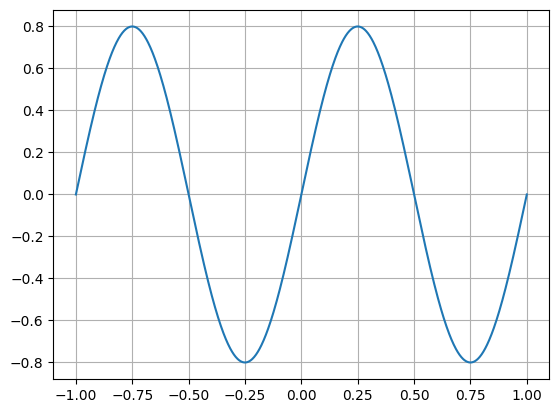
\includegraphics[width= 0.8\linewidth]{sine_wave.png}
        \caption{Sinusoidal modulating signal}
        %\label{fig:enter-label}
    \end{figure}
\end{frame}

\begin{frame}{Sine Triangle PWM}
\begin{itemize}
    \item $V_c(t) = \begin{cases}4tf_{2}-1&0\leq t\leq\frac{1}{2f_{2}}\\
    3 - 4tf_2&\frac{1}{2f_2}\leq t\leq\frac{1}{f_{2}}\end{cases} \quad for \quad0\leq t\leq\frac{1}{f_{2}}$\\
    periodic with period = $\frac{1}{f_2}$
\end{itemize}
    \begin{figure}
        \centering
        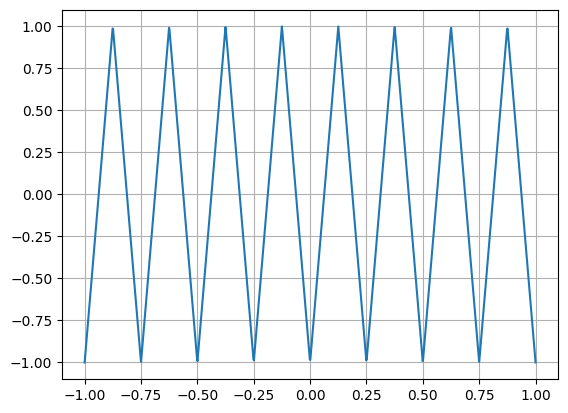
\includegraphics[width= 0.6\linewidth]{triangle_wave.png}
        \caption{Triangular Carrier Signal}
        %\label{fig:enter-label}
    \end{figure}
\end{frame}
\begin{frame}{Sine Triangle PWM}
    \begin{itemize}
        \item $V(t) = \begin{cases}
            1&V_m(t) \geq V_c(t)\\
            0& otherwise
        \end{cases}$
    \end{itemize}
    \begin{figure}
        \centering
        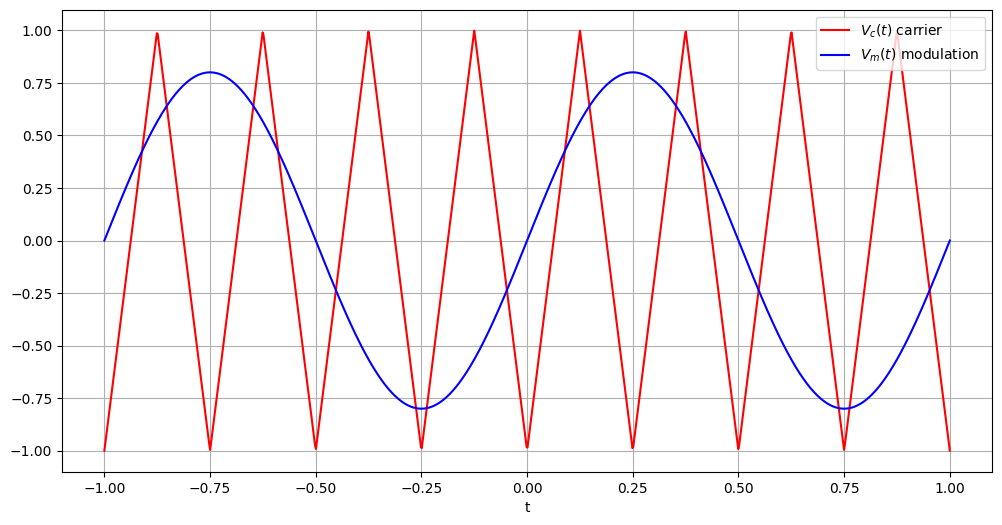
\includegraphics[width= 0.7\linewidth]{pwm.png}
        \caption{$V_m\quad and \quad V_c$}
        % \label{fig:enter-label}
    \end{figure}
\end{frame}
\begin{frame}{Sine Triangle PWM}
    \begin{figure}
        \centering
        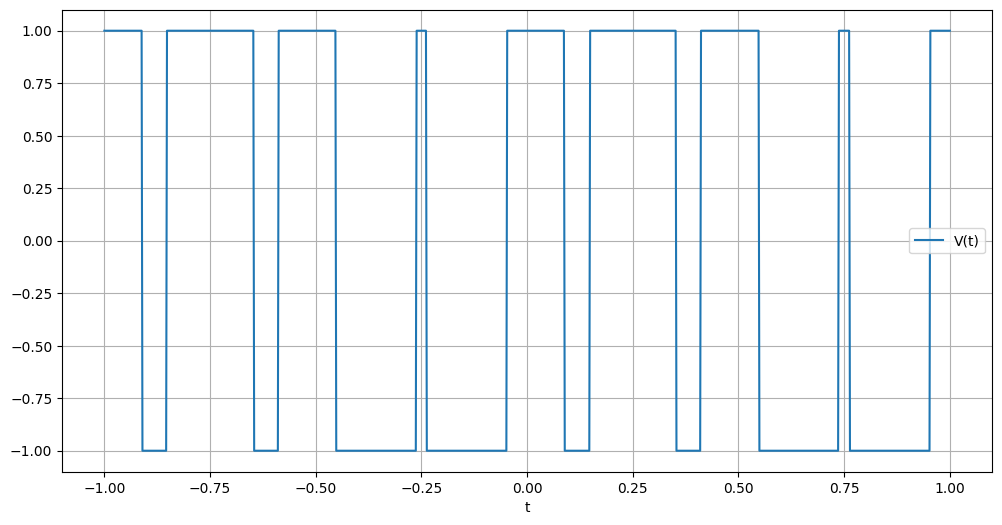
\includegraphics[width= 0.8\linewidth]{square_pwm.png}
        \caption{$V(t)$}
        % \label{fig:enter-label}
    \end{figure}
\end{frame}

\begin{frame}{Double Fourier Series of Sine Triangle PWM}
\begin{itemize}
    \item $X(T) = sin(2\pi T)$\\
    \begin{figure}
        \centering
        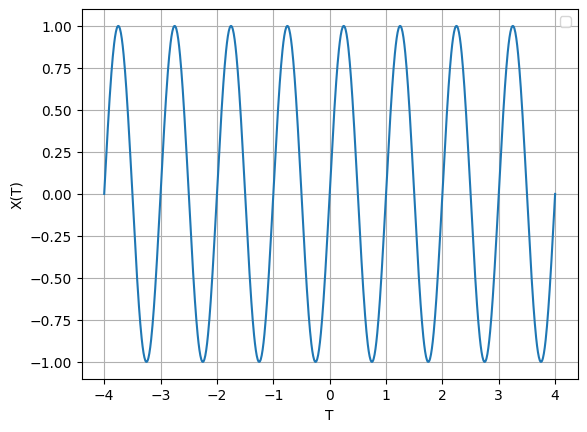
\includegraphics[width= 0.8\linewidth]{X_T.png}
    \end{figure}
    \item $X(T+1) = X(T)$
\end{itemize}
\end{frame}
\begin{frame}{Double Fourier Series of Sine Triangle PWM}
\begin{itemize}
    \item $Y(T) = \begin{cases}
            4T-1&0 \leq T \leq 1/2\\
            3-4T&1/2 \leq T \leq 1
        \end{cases}
        \quad \text{for} \quad 0 \leq T \leq 1$
    \begin{figure}
        \centering
        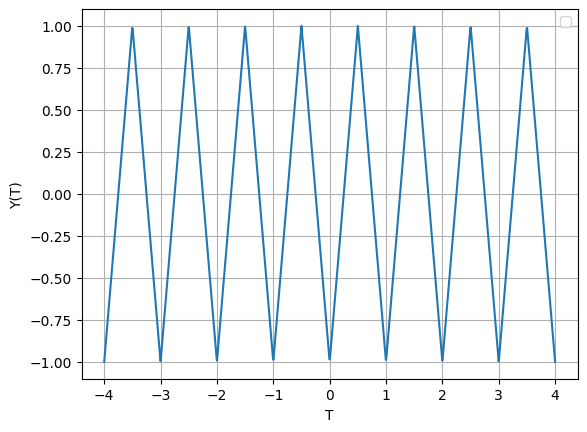
\includegraphics[width= 0.7\linewidth]{Y_T.png}
    \end{figure}
    \item Y(T+1) = Y(T)
\end{itemize}
\end{frame}

\begin{frame}{Double Fourier Series of Sine Triangle PWM}
    \begin{itemize}
        \item $V_m(t) = X(f_1t)$
        \item $V_c(t) = Y(f_2t)$
        \item $V(t) = \begin{cases}
            1&X(f_1t) \geq Y(f_2t)\\
            0& otherwise
        \end{cases}$
        \item Define
        \begin{align*}
            f(x,y) = \begin{cases}
                1&X(x) \geq Y(y)\\
                0& otherwise
            \end{cases}
        \end{align*}
        \item $f(x+1,y) = f(x,y+1) = f(x,y)$ 
    \end{itemize}
\end{frame}

\begin{frame}{Double Fourier Series of Sine Triangle PWM}
    \begin{itemize}
        \item Now, $V(t) = f(f_1t, f_2t)$
        \item Fourier series of f is
        \begin{align*}
            f(f_1t,f_2t) = a_{0}+ \sum b_{m}(2\pi mf_1t)+\sum c_{m}\sin(2\pi mf_1t)\\
            &\hspace{-17em} +\sum d_{n}\cos\left(2\pi nf_2t\right)+\sum e_{n}\sin\left(2\pi nf_2t\right)\\
            &\hspace{-17em} +\sum\sum f_{mn}\cos\left(2\pi mf_1t\right)\sin\left(2\pi nf_2t\right)\\
            &\hspace{-17em} +\sum\sum g_{mn}\cos\left(2\pi mf_1t\right)\cos\left(2\pi nf_2t\right)\\
            &\hspace{-17em} +\sum\sum h_{mn}\sin\left(2\pi mf_1t\right)\sin\left(2\pi nf_2t\right)\\
            &\hspace{-17em} +\sum\sum k_{mn}\sin\left(2\pi mf_1t\right)\cos\left(2\pi nf_2t\right)
        \end{align*}
    \end{itemize}
\end{frame}

\begin{frame}{Double Fourier Series of Sine Triangle PWM}
    \begin{itemize}
        \item \begin{align*}
            f(f_1t,f_2t) = a_{0}+ \sum b_{m}\cos(2\pi mf_1t)+\sum c_{m}\sin(2\pi mf_1t)\\
            &\hspace{-17em} +\sum d_{n}\cos\left(2\pi nf_2t\right)+\sum e_{n}\sin\left(2\pi nf_2t\right)\\
            &\hspace{-17em} +\sum_{m}\sum_{n}\sin\left(2\pi\left(nf_{2}+mf_{1}\right)t\right)\left(\frac{f_{mn}}{2}+\frac{k_{mn}}{2}\right)\\
            &\hspace{-17em}+\sum_{m}\sum_{n}\sin\left(2\pi\left(nf_{2}-mf_{1}\right)t\right)\left(\frac{f_{mn}}{2}-\frac{k_{mn}}{2}\right)\\
            &\hspace{-17em} +\sum_{m}\sum_{n}\cos\left(2\pi\left(nf_{2}+mf_{1}\right)t\right)\left(\frac{g_{mn}}{2}-\frac{h_{mn}}{2}\right)\\
            &\hspace{-17em} +\sum_{m}\sum_{n}\cos\left(2\pi\left(nf_{2}-mf_{1}\right)t\right)\left(\frac{g_{mn}}{2}+\frac{h_{mn}}{2}\right)
        \end{align*}
    \end{itemize}
\end{frame}

\begin{frame}{Double Fourier Series of Sine Triangle PWM}
\begin{itemize}
    \item $\sum b_{m}\cos(2\pi mf_1t)+\sum c_{m}\sin(2\pi mf_1t)$ is Harmonics from modulation signal
    \item $\sum d_{n}\cos\left(2\pi nf_2t\right)+\sum e_{n}\sin\left(2\pi nf_2t\right)$ is Harmonics from Carrier Signal
    \item $\sum_{m}\sum_{n}\sin\left(2\pi\left(nf_{2}+mf_{1}\right)t\right)\left(\frac{f_{mn}}{2}+\frac{k_{mn}}{2}\right) +\sum_{m}\sum_{n}\sin\left(2\pi\left(nf_{2}-mf_{1}\right)t\right)\left(\frac{f_{mn}}{2}-\frac{k_{mn}}{2}\right)+\sum_{m}\sum_{n}\cos\left(2\pi\left(nf_{2}+mf_{1}\right)t\right)\left(\frac{g_{mn}}{2}-\frac{h_{mn}}{2}\right) +\sum_{m}\sum_{n}\cos\left(2\pi\left(nf_{2}-mf_{1}\right)t\right)\left(\frac{g_{mn}}{2}+\frac{h_{mn}}{2}\right)$ are Sideband Harmonics
\end{itemize}
    
\end{frame}
\end{document}
